\documentclass{beamer}




\usepackage[T1,T2A]{fontenc}
\usepackage[utf8]{inputenc}

\usepackage{graphicx}
\usepackage{blindtext}
\usepackage{ mathrsfs }
\usepackage[russian,english]{babel}
%\usepackage{ dsfont }

\author{Деркач Максим Юрьевич}
\title{Криптографические протоколы}
\subtitle{AE-, AEAD-режимы шифрования}
\setbeamercolor{frametitle}{bg=cyan!10}


%\usetheme{lucid}
\begin{document}
	\frame {
		\titlepage
	}
	\frame {
		\frametitle{Ссылки}
		
		\url{https://www.cs.jhu.edu/~Eastubble/dss/ae.pdf}
		\url{http://cseweb.ucsd.edu/~mihir/papers/oem.pdf}
		\url{https://habr.com/en/post/425637/}
				
			
	}
	\frame{
		\frametitle{Введение}
		\textbf{AEAD-режим блочного шифрования (Authenticated Encryption with Associated Data)} — класс блочных режимов шифрования, при котором часть сообщения шифруется, часть остается открытой, и всё сообщение целиком аутентифицировано.
		
		\
		
		AEAD пришел на замену режиму AE(Authenticated Encryption), который используется/использовался в таких протоколах как (IPSEC, TLS, SSH...).
			
	}

	\frame{
	\frametitle{AE-режим}
		Шифрование с проверкой подлинности обеспечивает конфиденциальность и целостность данных для защищаемой информации. \\
		\bigskip
		
		
		Сущетвует три метода реализации AE-режима:
		\begin{enumerate}
			\item Authentication and Encryption (MacAndEnc)
			\item Authentication Then Encryption (MacThenEnc)
			\item Encryption Then Authentication (EncThenMac)
		\end{enumerate}
	
		\begin{table}[ht!]
		\begin{tabular}{llll}
			Метод &  Пример & Реализация & Результат\\
			MacAndEnc & SSH & $h = MAC(m), C = Enc(m)$ & $C||h$ \\ 
			MacThenEnc & SSL & $h = MAC(C), C = Enc(m || h)$ & $C$ \\
			EncThenMac & IPSEC & $C = Enc(m), h = MAC(C)$ & $C||h$ \\
		\end{tabular}
		\end{table}
	}

\frame{
	\frametitle{Определения}
	\textbf{Неразличимость шифротекста(Ciphertext indistinguishability)} - это свойство многих систем шифрования. Если система обладает свойством неразличимости, то злоумышленник не сможет отличить пары шифротекстов, основываясь на открытых текстах, которые они шифруют.
	\\
	\bigskip
	\textbf{IND-CPA} - Hеразличимость для атак на основе подобранного открытого текста
	
	\textbf{IND-CCA} - Hеразличимость для атак на основе подобранного шифротекста

		
}

\frame{
	\frametitle{Определения}
	\textbf{IND-CPA}
	\begin{enumerate}
	\item Испытатель генерирует ключ $K$ и передает его злоумышленнику.
	\item Злоумышленник может выполнить полиномиально ограниченное число шифрований.
	\item Злоумышленник представляет два отдельных открытых текста $M_0, M_1$ испытателю.
	\item Испытатель выбирает $b \in \{0, 1\}$ случайным образом и посылает шифротекст $C = E_K(M_b)$ обратно злоумышленнику.
	\item Злоумышленник может выполнять любое количество дополнительных вычислений или шифрований, и в конце выводит $b$.
	\end{enumerate}
	
	Криптосистема надёжна в смысле IND-CPA, если любой вероятный злоумышленник за полиномиальное время имеет лишь незначительное "преимущество" в различении шифротекстов над случайным угадыванием. 	
}

\frame{
	\frametitle{Определения}
	\textbf{IND-CCA}
	\begin{enumerate}
		\item -||-
		\item Злоумышленник может выполнить полиномиально ограниченное число шифрований и вызовов дешифрования с оракулом на основе произвольных шифротекстов.
		\item -||-
		\item -||-
		\item Злоумышленник может выполнять любое количество дополнительных вычислений или шифрований и:
		\begin{enumerate}
			\item (IND-CCA1) злоумышленник не может выполнять дальнейшие расшифрования с оракулом.
			\item (IND-CCA2) злоумышленник может выполнять дальнейшие вызовы оракула, но не может использовать для этого шифротекст $C$.
		\end{enumerate}	
		\item -||-
	\end{enumerate}

	$IND-CCA2 \Rightarrow IND-CCA1 \Rightarrow IND-CPA$
}

\frame{
	\frametitle{Определения}
	\textbf{Неизменяемость шифротекста(Non-Malleability)} - это свойство шифрования. Алгоритм шифрования является изменяемым («податливым»), если возможно преобразовать зашифрованный текст в другой зашифрованный текст, который расшифровывается в заданный открытый текст.
}

\frame{
	\frametitle{Определения}
	\textbf{Целостность открытого текста(INT-PTXT)} - это свойство означает, что невозможно создать такой шифротекст, что полученый при его расшифровке открытй текст отправитель никогда не отправлял (шифровал).
	\bigskip
	
	\textbf{Целостность открытого текста(INT-CTXT)} - это свойство означает, что невозможно создать шифротекст, ранее не созданый отпарвителем, независимо от того, являеться ли базовый секрет(откртый текст) новым.
	
	$INT-CTXT \Rightarrow INT-PTXT$
}
	\frame{
	\frametitle{AE-режим}
	Сравнение  AE-режимов:
	\bigskip
	
	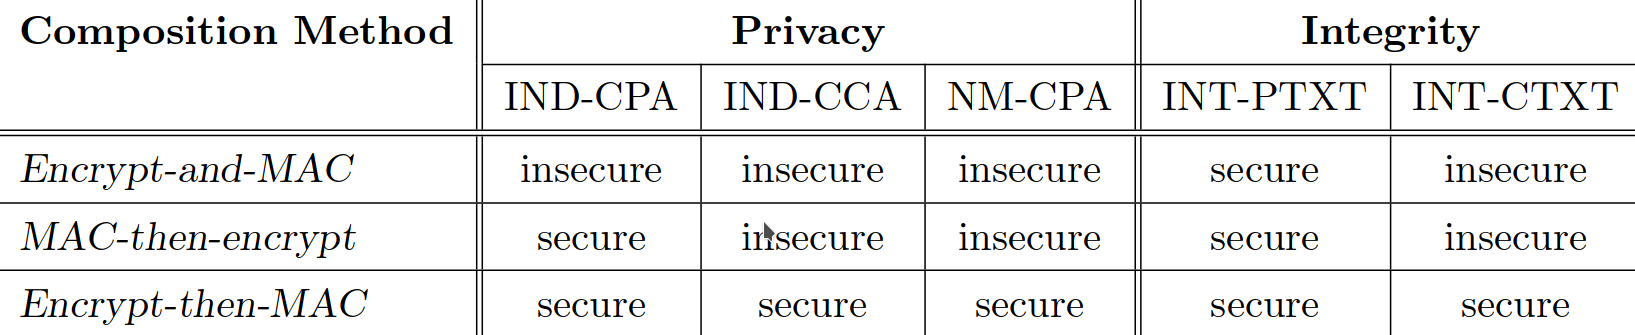
\includegraphics[width=0.8\linewidth]{mac.png}

}
	\frame{
	\frametitle{AEAD-режим}
		Сущетвует 2 метода реализации AE-режима:
		\begin{enumerate}
			\item С помощью алгоритмов EncThenMac и MacThenEnc.
			\item С помощью модификации AE-режима.
		\end{enumerate}
	\bigskip
	$H$ - открытый загаловок; $M$ - сообщение; $N$ - nonce; $E$ - симметричная к/c; $F$ -  MAC-алгоритм;
	\includegraphics[width=0.4\linewidth]{Encrypt-Then-mac.png}
	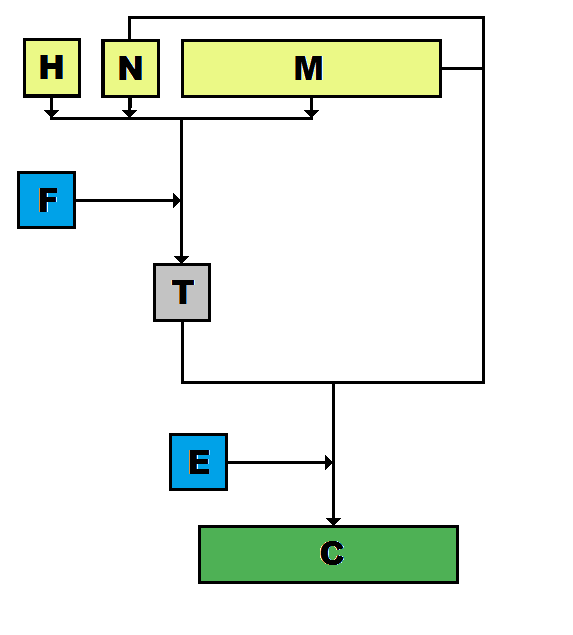
\includegraphics[width=0.4\linewidth]{Mac-then-encrypt.png}	
	
	}
	
	\frame{
		\frametitle{AEAD-режим}
		Примеры модификации AE-режима:
		\begin{enumerate}
			\item Nonce stealing. \\
			Открытый загаловок передается внутри поля nonce.
			\item Ciphertext translation. 
			$\hat{E}(K, K_{MAC}, N, M, H)= E_K(N,M)\oplus MAC_{K_{MAC}}(H)$
			
			$\hat{D}(K, K_{MAC}, N, C, H)= D_K(N, C \oplus MAC_{K_{MAC}}(H))$,\\
			
			где $E, D$ - шифрование и дешифрование в режиме AE.
			
		\end{enumerate}
		
	}
	

	\frame {
	\begin{figure}
		%
\includegraphics[width=0.8\linewidth]{memes1.jpeg}
		
	\end{figure}
	}

\end{document}